% Drawing 64/01-1 -- folder 64, batch 01, archive page 12 (PDF page 13).
% Transcription: marge gauche, en haut : un carré dont l'arête inférieure $a$ et l'arête supérieure $a'$ sont épaissies, le sommet $s$ en bas à gauche (gros point) et le sommet $s'$ en haut à droite, et la diagonale $d$ tracée de $s$ à $s'$.
% Kind: square with two heavy edges and a diagonal (frame of the cube on a face). Method 2 (schematic redraw from the facsimile). Status: ok.
% Notes: As on the page: the square, its lower edge a and its upper edge a' heavy, the two other sides lighter, the diagonal d from s (lower left, heavy point) to s' (upper right), the five letters where he wrote them. All edges and the diagonal are drawn between the same four vertices. Nothing struck. Redrawn 2026-11-12 (issue 128): to check again.
% Coordinates: 1 unit = 0.4 mm = 1/100 of the crop width (bbox in page fractions: [0.1, 0.19, 0.2, 0.26]).
% Redrawn by Claude (claude-fable-5-2), issue #128, 2026-11-12; not checked by a human; not compiled (no TeX in the session).
% Rights: reproduces part of the work -- behind RENDER_TRANSCRIPTS, never published by itself.
\documentclass[tikz,border=3pt]{standalone}
\usepackage{amsmath,amssymb}
\usetikzlibrary{patterns,arrows.meta}
\tikzset{pencil/.style={black!45}, struck/.style={black!35}, mpt/.style={circle,draw,inner sep=1.3pt}, pt/.style={circle,fill,inner sep=0.9pt}, opt/.style={circle,draw,fill=white,inner sep=1.1pt}}
\begin{document}
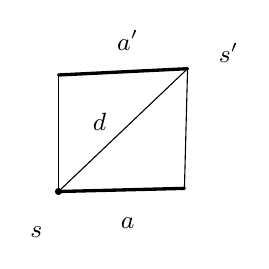
\begin{tikzpicture}[x=0.4mm,y=0.4mm,line cap=round,line join=round,font=\scriptsize]
\draw[very thick] (26,-40) -- (67,-38);
\draw[very thick] (26,-77) -- (66,-76);
\draw (26,-40) -- (26,-77);
\draw (67,-38) -- (66,-76);
\draw (26,-77) -- (67,-38);
\node[pt] at (26,-77) {};
\node[inner sep=1pt] at (48,-29) {\small $a'$};
\node[inner sep=1pt] at (80,-33) {\small $s'$};
\node[inner sep=1pt] at (39,-55) {\small $d$};
\node[inner sep=1pt] at (19,-90) {\small $s$};
\node[inner sep=1pt] at (48,-87) {\small $a$};
\end{tikzpicture}
\end{document}
